% SC4063 --- Chapter 6: Wireless Security --- WEP, WPA2, WPA3 and Evil Twins (0->100)
% No \documentclass --- this file is \include'd by main.tex (book class).
\chapter{Wireless Security: WEP, WPA2, WPA3 and Evil Twins}\label{ch:wireless}
\begin{quote}
\emph{``If the medium is air, the adversary owns the air around you.''} --- A cable is a private hallway; Wi-Fi is a shout across a caf\'e. Anyone nearby can listen, and anyone who shouts louder can pretend to be the caf\'e.
\end{quote}

\noindent\fbox{\parbox{\dimexpr\linewidth-2\fboxsep-2\fboxrule}{%
\textbf{From zero: no wireless background assumed.} We start from a radio broadcast where every nearby receiver hears every frame. From that intuition we ask: how do we give a private conversation over a public shout, why the first attempt (WEP) failed catastrophically, how WPA2 fixed it but still left a handshake crack, and how WPA3 tries to fix that too. One picture at a time: cipher, handshake, impersonation.}}
\vspace{0.4em}

\section*{Learning Outcomes}
After this chapter you will be able to:
\begin{enumerate}[label=(L\arabic*)]
    \item explain why wireless amplifies eavesdropping, injection and impersonation compared to wired;
    \item describe WEP's RC4/CRC design and enumerate its three fatal flaws;
    \item trace the WPA2 4-way handshake, CCMP's AES-CCM, and the KRACK reinstall;
    \item compare WPA3-Personal (SAE), WPA3-Enterprise 192-bit, OWE and PMF with WPA2;
    \item design and detect an evil-twin / rogue AP attack and propose mitigation.
\end{enumerate}

% ============================================================
{\sloppy
\section{Air Is Broadcast}\label{sec:air}
On Ethernet a frame traverses a wire between two ports; on 802.11 it radiates. Any antenna in range ($\approx 30$\,m indoors, $>200$\,m with a dish) receives every frame, regardless of destination. The header (BSSID, source/destination MAC, sequence number) is never encrypted, even when the payload is. An attacker can passively map SSIDs, count clients, measure signal to locate devices, and inject frames by waiting for a clear channel. Confidentiality, integrity and authenticity must be retrofitted onto this broadcast.

A \emph{master secret} (pre-shared key or enterprise credential) must be stretched into fresh session keys per association, and those keys must be proven without revealing them over the air. That proof is the handshake.

\section{WEP: A Case Study in How Not To}\label{sec:wep}
WEP (1997) used RC4 with a 40- or 104-bit key plus a 24-bit IV prepended in clear: keystream $=$ RC4(key $\\Vert$ IV), ciphertext $=$ plaintext $\oplus$ keystream, integrity $=$ CRC-32 (linear, not cryptographic). Three breaks, each fatal alone:

\begin{description}[leftmargin=1.2em, itemsep=0.3em]
    \item[Small IV, no replay protection] 24\,bit $\to$ $2^{24}\approx16$\,M values. A busy AP cycles the IV in hours; collisions reuse the same keystream. XOR of two ciphertexts with the same IV is XOR of plaintexts---English text breaks quickly.
    \item[RC4 weak keys + related-key] The first bytes of RC4 keystream leak key bits (Fluhrer--Mantin--Shamir, 2001). With $\approx40\,000$ frames an attacker recovers the key passively.
    \item[Linear CRC] Flipping a bit and fixing the CRC is trivial; integrity checks nothing against an active attacker.
\end{description}

Tools like \texttt{aircrack-ng} automated this to minutes by 2005. WEP is not ``weak''; it is broken by design. Never use it, even for ``low-value'' traffic.

\begin{center}
\begin{tikzpicture}[scale=0.84, every node/.style={font=\scriptsize}]
  \node[draw, fill=red!16, rounded corners, minimum width=2.3cm, minimum height=1.0cm, align=center] (wep) at (0,0) {WEP (1997)\\ \tiny RC4, 24-bit IV\\Cracked $>$2001};
  \node[draw, fill=orange!18, rounded corners, minimum width=2.7cm, minimum height=1.0cm, align=center] (wpa2) at (4.2,0) {WPA2 (2004)\\ \tiny CCMP/AES, 4-way\\KRACK 2017};
  \node[draw, fill=green!16, rounded corners, minimum width=2.7cm, minimum height=1.0cm, align=center] (wpa3) at (8.4,0) {WPA3 (2018)\\ \tiny SAE, PMF, OWE\\128/192-bit};
  \draw[->, thick, red!60!black] (wep.east) -- (wpa2.west) node[midway,above,font=\tiny] {TKIP bridge};
  \draw[->, thick, orange!60!black] (wpa2.east) -- (wpa3.west) node[midway,above,font=\tiny] {Dragonfly};
  \node[below=0.40cm of wep, font=\tiny, text=red!70!black] {minutes};
  \node[below=0.40cm of wpa2, font=\tiny, text=orange!70!black] {offline dict.};
  \node[below=0.40cm of wpa3, font=\tiny, text=green!60!black] {forward secrecy};
  \draw[decorate, decoration={brace,mirror,amplitude=4pt}, thick] (-1.3,-1.05) -- (10.0,-1.05) node[midway,below=4pt,font=\tiny] {each generation fixes the handshake, not just the cipher};
\end{tikzpicture}
\end{center}

WPA (2003) was a TKIP band-aid that still used RC4; WPA2 (2004) finally mandated AES.

\section{WPA2: Handshake and CCMP, Then KRACK}\label{sec:wpa2}
WPA2-Personal derives a Pairwise Master Key PMK $=$ PBKDF2(passphrase, SSID, 4096). The 4-way handshake proves possession of the PMK and negotiates fresh PTK/GTK without sending the PMK over the air, and installs the key for CCMP (AES in CCM mode: authenticated encryption).

\begin{center}
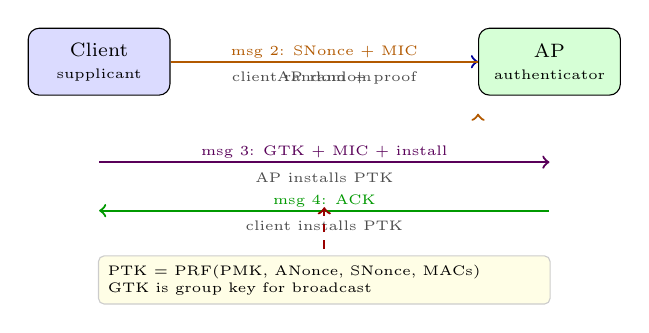
\begin{tikzpicture}[scale=0.88, every node/.style={font=\scriptsize}]
  \node[draw, fill=blue!14, rounded corners, minimum width=1.8cm, minimum height=0.85cm, align=center] (sta) at (0,3.0) {Client\\ \tiny supplicant};
  \node[draw, fill=green!16, rounded corners, minimum width=1.8cm, minimum height=0.85cm, align=center] (ap) at (6.5,3.0) {AP\\ \tiny authenticator};
  \draw[->, thick, blue!60!black] (sta.east) -- (ap.west) node[midway,above,font=\tiny, fill=white, inner sep=1pt] {msg 1: ANonce} node[midway,below,font=\tiny, text=gray!60!black] {AP random};
  \draw[<-, thick, orange!70!black] (sta.east) -- (ap.west) ++(0,-0.75) node[midway,above,font=\tiny, fill=white, inner sep=1pt] {msg 2: SNonce + MIC} node[midway,below,font=\tiny, text=gray!60!black] {client random + proof};
  \draw[->, thick, violet!70!black] (0,1.55) -- (6.5,1.55) node[midway,above,font=\tiny, fill=white, inner sep=1pt] {msg 3: GTK + MIC + install} node[midway,below,font=\tiny, text=gray!60!black] {AP installs PTK};
  \draw[<-, thick, green!60!black] (0,0.85) -- (6.5,0.85) node[midway,above,font=\tiny, fill=white, inner sep=1pt] {msg 4: ACK} node[midway,below,font=\tiny, text=gray!60!black] {client installs PTK};
  \node[font=\tiny, fill=yellow!10, draw=gray!40, rounded corners=2pt, align=left, text width=5.5cm] at (3.25,-0.15) {PTK = PRF(PMK, ANonce, SNonce, MACs)\\GTK is group key for broadcast};
  \draw[->, thick, dashed, red!60!black] (3.25,0.30) -- (3.25,0.90);
\end{tikzpicture}
\end{center}

CCMP then encrypts each 802.11 data frame with a 48-bit packet number (PN) as nonce: replay is detected when PN does not increase, and tampering is caught by the CCM MIC. This fixed WEP's crypto.

KRACK (Vanhoef--Piessens, 2017) did not break AES; it broke the \emph{handshake state machine}. By replaying msg~3, the attacker forced the client to reinstall an already-used PTK, resetting PN and keystream. With keystream reuse, the attacker could decrypt and inject. The fix is to forbid reinstall of the same key and to use a single PN counter across installs. PMF (802.11w) helps: it protects deauthentication frames that KRACK abused to force reconnects.

Offline dictionary remains WPA2-Personal's practical weakness. The 4-way handshake's MIC gives an offline verifier for passphrases; a captured handshake plus a wordlist (or GPU brute-force at $\approx 10^9$ PBKDF2/sec on modern GPUs) cracks weak passwords. Enterprise mode avoids this by using 802.1X/EAP-TLS with per-user credentials.

\begin{lstlisting}[language=bash,caption={Capturing a WPA2 handshake and testing a passphrase list.},label={lst:wpa2-crack}]
# Put card in monitor, capture handshake on channel 6
sudo airmon-ng start wlan0           # -> wlan0mon
sudo airodump-ng -c 6 --bssid AA:BB:CC:DD:EE:FF -w capture wlan0mon
# Deauth a client to force a fresh handshake (lab only, with permission)
sudo aireplay-ng --deauth 5 -a AA:BB:CC:DD:EE:FF wlan0mon
# Crack offline: only works for weak passphrases
aircrack-ng -w rockyou.txt capture-01.cap
# Mitigation check: is PMF required? (802.11w)
iw dev wlan0 scan | grep -i "PMF"
\end{lstlisting}

\section{WPA3: SAE, Forward Secrecy and OWE}\label{sec:wpa3}
WPA3-Personal replaces the 4-way handshake's PSK proof with \emph{Simultaneous Authentication of Equals} (SAE, Dragonfly): a zero-knowledge password-authenticated key exchange. An attacker who captures the handshake learns nothing for offline dictionary; they must \emph{interact} for each guess, and the AP can rate-limit. SAE also gives \emph{forward secrecy}: compromising the password later does not decrypt past captures. Transition mode (WPA2+WPA3 on the same SSID) keeps compatibility but downgrade attacks are possible if not configured to prefer WPA3.

For open networks, WPA3 adds \emph{Opportunistic Wireless Encryption} (OWE, RFC~8110): unauthenticated encryption---no passphrase, but every client gets a fresh key so passive sniffing is defeated. The caf\'e AP finally encrypts even when there is no password; authentication is still absent (evil twin still possible).

WPA3-Enterprise offers a 192-bit suite (GCMP-256, HMAC-SHA-384) and mandates PMF. Together, SAE $+$ PMF $+$ OWE close the three WPA2 gaps: offline dictionary, deauth, and open-network sniffing.

\begin{remark}[Dragonblood and transition pains]\label{rem:dragonblood}
WPA3 did not ship flawlessly. Dragonblood (Vanhoef--Ronen, 2019) showed side-channel and downgrade issues in early SAE implementations: timing and cache attacks leaked password bits, and a transition-mode AP that offered both WPA2 and WPA3 could be downgraded to the weaker handshake by spoofing beacons. The fixes were firmware upgrades and an anti-clogging token plus constant-time hunting-and-pecking. Lesson: even a formally verified handshake (SAE is based on a balanced PAKE) can fail in code that is not constant-time. Deploy WPA3 only with patched firmware and set \texttt{sae\_require\_mfp=1} to forbid downgrade where possible. Transition mode is a bridge, not a destination.
\end{remark}

\section{Evil Twin and Rogue AP}\label{sec:evil}
An \emph{evil twin} copies a legitimate SSID/BSSID (often with higher TX power) and lures clients that auto-join by SSID alone. With \texttt{hostapd} plus \texttt{dnsmasq} the attacker runs a full AP on a laptop, serves a captive portal, and relays or strips traffic. Enterprise (EAP-TLS) resists the twin because the client validates the \emph{server's certificate}, not just the SSID. Pre-shared-key networks have no such anchor.

\begin{center}
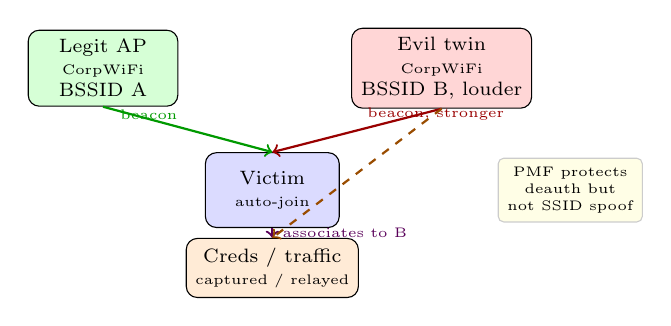
\begin{tikzpicture}[scale=0.86, every node/.style={font=\scriptsize}]
  \node[draw, fill=green!16, rounded corners, minimum width=1.9cm, minimum height=0.95cm, align=center] (legit) at (0,1.8) {Legit AP\\ \tiny CorpWiFi\\BSSID A};
  \node[draw, fill=red!16, rounded corners, minimum width=1.9cm, minimum height=0.95cm, align=center] (evil) at (5.0,1.8) {Evil twin\\ \tiny CorpWiFi\\BSSID B, louder};
  \node[draw, fill=blue!14, rounded corners, minimum width=1.7cm, minimum height=0.95cm, align=center] (vic) at (2.5,0) {Victim\\ \tiny auto-join};
  \node[draw, fill=orange!16, rounded corners, minimum width=1.7cm, minimum height=0.75cm, align=center] (cred) at (2.5,-1.15) {Creds / traffic\\ \tiny captured / relayed};
  \draw[->, thick, green!60!black] (legit.south) -- (vic.north) node[midway,above left,font=\tiny] {beacon};
  \draw[->, thick, red!60!black] (evil.south) -- (vic.north) node[midway,above right,font=\tiny] {beacon, stronger};
  \draw[->, thick, violet!70!black] (vic.south) -- (cred.north) node[midway,right,font=\tiny] {associates to B};
  \draw[->, thick, dashed, orange!60!black] (evil.south) -- (cred.north);
  \node[font=\tiny, fill=yellow!10, draw=gray!40, rounded corners=2pt, align=center] at (6.9,0) {PMF protects\\deauth but\\not SSID spoof};
\end{tikzpicture}
\end{center}

Detection: monitor for duplicate BSSIDs with divergent capabilities (PMF required vs.\ not, differing RSSI jumps, unexpected channel, new OUI). Enterprise tools (WIDS/WIPS) triangulate rogues; on Linux:

\begin{lstlisting}[language=bash,caption={Rogue AP detection with signal and capability anomaly.},label={lst:evil-detect}]
# Scan and flag SSIDs seen with >1 BSSID or capability mismatch
sudo iw dev wlan0 scan | awk '/BSS/{b=$2} /SSID:/{s=$2} /RSN:/{r=$0} {print b,s,r}' | sort | uniq -c | awk '$1>1'
# Continuous monitor: alert on deauth floods (PMF should protect)
sudo tshark -i wlan0mon -Y "wlan.fc.type_subtype==12" -T fields -e wlan.sa -e wlan.da | sort | uniq -c | sort -nr | head
# Prefer WPA3/OWE and pin expected BSSID where possible
# wpa_supplicant: bssid_allowlist=aa:bb:cc:dd:ee:ff  (lab pinning)
\end{lstlisting}

Mitigations ladder: for new deployments use WPA3-Enterprise with EAP-TLS (certificate pinning kills the twin), or WPA3-Personal with a strong random 20+ character passphrase and PMF required. For existing WPA2-PSK, rotate to a long passphrase, disable WPS, enable PMF if clients support it, and educate against auto-joining open or known SSIDs. For open hospitality, deploy OWE so even unauthenticated encryption raises the bar.

\section{Putting It Together: Hardening Checklist}\label{sec:hardening}
Wireless hardens in layers, mirroring the firewall ladder of Ch.~2. Use this checklist when you audit a deployment:

\begin{enumerate}[leftmargin=1.4em, itemsep=0.35em]
    \item \textbf{Choose the suite per SSID.} Employee: WPA3-Enterprise/EAP-TLS, 192-bit, PMF required. Guest: OWE (or WPA3-Personal with a daily rotating 20-char passphrase displayed at reception). Never mix WEP/WPA with the same SSID.
    \item \textbf{Require PMF and disable downgrade.} Set \texttt{pmf=2} (required) on the AP; clients that cannot do PMF are upgraded, not accommodated. In transition mode, prefer WPA3 and log WPA2 associations for upgrade tracking.
    \item \textbf{Manage the secret.} For PSK, generate with \texttt{pwgen 24 1} and rotate quarterly; for Enterprise, provision per-user certificates via MDM and revoke on off-boarding. Disable WPS (PIN is brute-forceable in $<$10\,hours).
    \item \textbf{Detect rogues continuously.} Deploy a WIDS sensor per floor (or use AP's built-in WIDS) that alerts on new BSSID+SSID pairs, PMF mismatch, and deauth floods. Feed alerts to the SIEM (Ch.~7).
    \item \textbf{Segment wireless from wired.} Terminate Wi-Fi on a controller in the DMZ; firewall the controller$\to$core at L3. A compromised wireless client should not see the DB VLAN without an additional VPN/802.1X hop.
\end{enumerate}

\begin{center}
\begin{tikzpicture}[scale=0.84, every node/.style={font=\scriptsize}]
  \node[draw, fill=red!14, rounded corners, minimum width=2.0cm, minimum height=0.8cm, align=center] (c1) at (0,0) {Weak\\ \tiny WEP / WPS};
  \node[draw, fill=orange!18, rounded corners, minimum width=2.0cm, minimum height=0.8cm, align=center] (c2) at (3.0,0) {WPA2-PSK\\ \tiny short pwd};
  \node[draw, fill=yellow!16, rounded corners, minimum width=2.0cm, minimum height=0.8cm, align=center] (c3) at (6.0,0) {WPA2-PSK\\ \tiny long + PMF};
  \node[draw, fill=green!16, rounded corners, minimum width=2.0cm, minimum height=0.8cm, align=center] (c4) at (9.0,0) {WPA3-Ent\\ \tiny EAP-TLS + PMF};
  \draw[->, thick] (c1.east) -- (c2.west);
  \draw[->, thick] (c2.east) -- (c3.west);
  \draw[->, thick] (c3.east) -- (c4.west);
  \node[below=0.40cm of c1, font=\tiny, text=red!70!black] {cracked};
  \node[below=0.40cm of c4, font=\tiny, text=green!60!black] {twin-resilient};
  \node[above=0.50cm of c2, font=\tiny, fill=yellow!10, draw=gray!40, rounded corners=2pt] {hardening ladder};
\end{tikzpicture}
\end{center}

\begin{lstlisting}[language=bash,caption={Hardening wpa\_supplicant and hostapd for WPA3 + PMF.},label={lst:hardening}]
# wpa_supplicant.conf -- prefer WPA3, require PMF, pin BSSID
network={
    ssid="CorpWiFi"
    key_mgmt=SAE                # WPA3-Personal; use WPA-EAP for Enterprise
    sae_password="correct-horse-battery-staple-24!"
    ieee80211w=2                # 2 = require PMF, 1 = optional
    bssid_allowlist=aa:bb:cc:dd:ee:ff
    scan_freq=2412 2437 2462
}
# hostapd.conf -- WPA3-Personal, PMF required, disable WPS
interface=wlan0
ssid=CorpWiFi
wpa=2
wpa_key_mgmt=SAE
wpa_passphrase=correct-horse-battery-staple-24!
ieee80211w=2
sae_require_mfp=1
wps_state=0                     # disable WPS PIN
\end{lstlisting}

\begin{remark}[Usability vs.\ security]
Every extra click pushes users toward workarounds (hotspots, tethering). OWE is the pragmatic win for open venues: zero friction, yet passive sniffing is defeated. For employee Wi-Fi, the MDM that silently provisions the EAP-TLS certificate is worth more than a 30-character PSK that users write on sticky notes.
\end{remark}

\begin{remark}[Wi-Fi 6E and the 6\,GHz mandate]
At 6\,GHz (Wi-Fi 6E) the Wi-Fi Alliance mandates WPA3; WPA2 is not allowed. Greenfield 6\,GHz deployments are thus WPA3-only by regulation, sidestepping transition-mode downgrade entirely. If you control the band, deploy there first and keep 2.4/5\,GHz as a legacy bridge with PMF logging. The 6\,GHz band is also where OWE becomes the default for ``open'' hospitality: encrypted by default, even when authentication is absent.
\end{remark}

\textit{Measurement tip:} Run \texttt{iw dev wlan0 station dump} on associated clients to see negotiated cipher (CCMP vs.\ GCMP) and PMF status; \texttt{hostapd\_cli sta} shows the AP's view. A mismatched \texttt{CCMP} vs.\ \texttt{GCMP-256} on a WPA3-Enterprise SSID is a client that needs a driver update before you can enforce 192-bit.

}

\section{Exercises}
\begin{exercise}WEP uses a 24-bit IV. A busy 802.11g AP sends 700 frames/sec. How long until IV collisions are expected (birthday bound $\approx \sqrt{2^{24}}$)? Why does this break confidentiality even though RC4 itself may be keyed correctly?\end{exercise}
\begin{exercise}Trace the WPA2 4-way handshake labelling ANonce, SNonce, PMK, PTK and GTK. At which message does the AP install the PTK? Explain how replaying message~3 in KRACK resets the packet number and why that leads to keystream reuse in CCMP.\end{exercise}
\begin{exercise}An 8-character lowercase password is used with WPA2-Personal (PBKDF2 4096 iterations). Estimate the search space and discuss whether a captured 4-way handshake can be cracked offline on a GPU testing $10^6$ passphrases/sec. How does WPA3 SAE change the answer? Include forward secrecy.\end{exercise}
\begin{exercise}Design an evil-twin lab (with permission): (a) write a \texttt{hostapd.conf} that clones an existing WPA2 SSID, (b) explain why a client that auto-joins open SSIDs is easier to bait than one that requires WPA3-Enterprise certificate validation, (c) list three detector signals a WIDS would use to flag your twin.\end{exercise}
\begin{exercise}A hotel offers \texttt{HotelWiFi} as open + captive portal. Compare (i) open, (ii) OWE, and (iii) WPA3-Personal with a per-room password for confidentiality, evil-twin resilience and usability. Recommend a deployment with PMF and explain the residual risk of a twin that also offers OWE.\end{exercise}


\textit{Lab note:} In a permissioned testbed, compare \texttt{aircrack-ng} time on WPA2-PSK (\texttt{rockyou.txt}, 14M) vs.\ WPA3-SAE where the same capture yields no offline verifier; the tool will report ``no valid handshake'' and each guess must be online, throttled to $\approx10$/s by the AP.
Transition captures also reveal the cost of crypto: CCMP adds 16\,B MIC + 8\,B header per MPDU; at 1500\,B MTU the overhead is $\approx1.6\%$ but the per-packet AES operation at $\sim$1\,Gbps is negligible on modern SoCs with AES-NI.
\section*{Chapter Notes}
WEP breaks are Fluhrer--Mantin--Shamir (2001) and Tews--Weinmann--Pyshkin (2007); CCMP and the 4-way handshake are 802.11-2016. KRACK is Vanhoef--Piessens (2017, CCS) and its PMF discussion is 802.11w-2009. WPA3/SAE/OWE are Wi-Fi Alliance (2018) and RFC~8110; 192-bit suite is Suite-B. Evil-twin tooling is \texttt{hostapd}, \texttt{airbase-ng} and \texttt{wifiphisher}; detection follows 802.11 -- Physical layer DoS and rogue-AP surveys (Bahl et al.).
% End of Chapter 6
% End of Chapter 6
